\section{The horizon reversal}
\label{sec:reversal}

\begin{figure}[t]
\centering
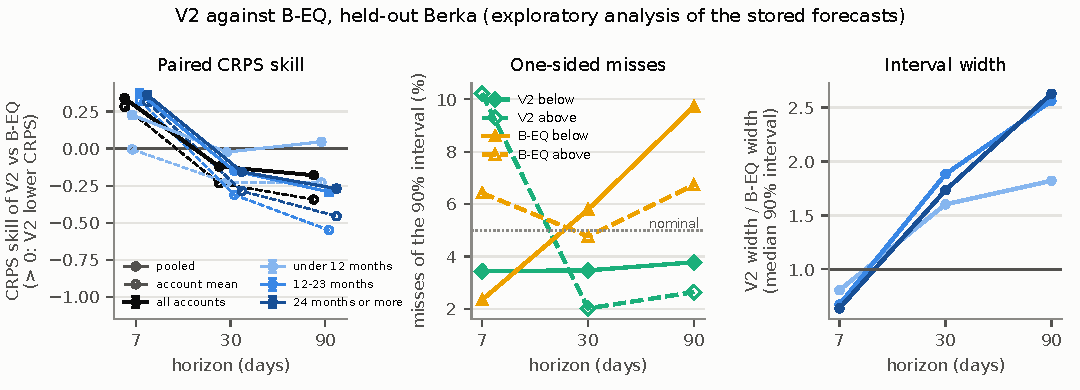
\includegraphics[width=\linewidth]{figures/reversal-heldout.pdf}
\caption{V2 against B-EQ on held-out Berka, from the stored forecasts of the
frozen evaluation; the history strata and one-sided misses are post hoc
(exploratory). Left: paired CRPS skill of V2 against B-EQ, for all
accounts and by months of history at the origin: pooled over origins
(filled, with \R{c/ci-level}\% account-bootstrap intervals) and the planned
mean of per-account ratios (open, dashed). Centre: the share of forecasts whose outcome
falls below or above the \lC\% interval (nominal: half the misses each).
Right: V2's median \lC\% interval width relative to B-EQ's. Origins:
\R{xh/s3/V2-vs-B-EQ/30/forecasts} per horizon in
\R{xh/s3/V2-vs-B-EQ/30/accounts} accounts; by stratum,
\R{xh/s3-history-lt12/V2-vs-B-EQ/30/forecasts} (under 12 months),
\R{xh/s3-history-12to23/V2-vs-B-EQ/30/forecasts} (12--23) and
\R{xh/s3-history-ge24/V2-vs-B-EQ/30/forecasts} (24 or more).}
\label{fig:reversal}
\end{figure}

\paragraph{The reversal.} On held-out accounts, V2 has lower CRPS than B-EQ
at \hA\ days and higher CRPS at \hB\ and \hC\ days
(Table~\ref{tab:pairwise}). The same holds under both aggregations.

\begin{center}\footnotesize
\begin{tabular}{lll}
\toprule
Horizon & Account-mean skill of V2 & Pooled skill of V2\\
\midrule
\hA\ days & \R{ho/pair/B-EQ/7/skill} [\R{ho/pair/B-EQ/7/skill_lo}, \R{ho/pair/B-EQ/7/skill_hi}] & \R{ho/pair/B-EQ/7/pooled_skill}\\
\hB\ days & \R{ho/pair/B-EQ/30/skill} [\R{ho/pair/B-EQ/30/skill_lo}, \R{ho/pair/B-EQ/30/skill_hi}] & \R{ho/pair/B-EQ/30/pooled_skill}\\
\hC\ days & \R{ho/pair/B-EQ/90/skill} & \R{ho/pair/B-EQ/90/pooled_skill}\\
\bottomrule
\end{tabular}
\end{center}

The mean CRPS behind the \hB-day comparison is \R{ho/pair/B-EQ/30/mean_crps_norm}
for V2 and \R{ho/pair/B-EQ/30/mean_crps_norm_ref} for B-EQ (normalized
units).

\paragraph{By history length, the two aggregations disagree}
(Figure~\ref{fig:reversal}, left; exploratory). Skill of V2 against B-EQ
at \hA, \hB\ and \hC\ days, pooled (account mean in brackets):
\begin{itemize}
  \item \textbf{Under a year of history:} \pq{xh/s3-history-lt12/V2-vs-B-EQ}{7},
  \pq{xh/s3-history-lt12/V2-vs-B-EQ}{30} and
  \pq{xh/s3-history-lt12/V2-vs-B-EQ}{90}.
  \item \textbf{24 months or more:} \pq{xh/s3-history-ge24/V2-vs-B-EQ}{7},
  \pq{xh/s3-history-ge24/V2-vs-B-EQ}{30} and
  \pq{xh/s3-history-ge24/V2-vs-B-EQ}{90}.
\end{itemize}
Pooled over origins, the long-horizon gap closes or reverses for short
histories. Under the plan's account mean it does not: B-EQ has lower CRPS
at \hB\ and \hC\ days even with under a year of history (account-mean
interval at \hC\ days
[\R{xh/s3-history-lt12/V2-vs-B-EQ/90/skill_mean_lo},
\R{xh/s3-history-lt12/V2-vs-B-EQ/90/skill_mean_hi}]).

B-EQ samples the account's past $h$-day changes. With a short history it
has few of them, and its long-horizon intervals under-cover: on accounts
with under a year of history, its \lC\% interval at \hC\ days covers
\R{ho/str/history-lt-12-months/B-EQ/90/cov90}\%, against V2's
\R{ho/str/history-lt-12-months/V2/90/cov90}\%.

\paragraph{Lower CRPS, narrower intervals, more misses below.} B-EQ's lower
CRPS at long horizons comes with intervals about half as wide as V2's.
\begin{itemize}
  \item \textbf{Median \lC\% width at \hC\ days:} \R{ho/var/B-EQ/90/median_width90_czk}
  CZK for B-EQ, against \R{ho/var/V2/90/median_width90_czk} for V2.
  \item \textbf{Misses below that interval:} \R{ho/tail/B-EQ/90/miss_low}\% for B-EQ,
  against V2's \R{ho/tail/V2/90/miss_low}\% (Figure~\ref{fig:reversal},
  centre).
\end{itemize}

V2 is the more cautious forecaster about the downside. B-EQ is the
sharper one, and on Berka its sharpness pays more in CRPS than its
under-coverage costs.

\begin{table}[t]
\centering\scriptsize\setlength{\tabcolsep}{3.5pt}
\tab{heldout-pairwise}
\caption{V2 against each baseline on held-out Berka, over the forecasts both
made (counts given). CRPS skill as the mean of per-account ratios (the
planned estimand) and as the pooled ratio over origins, each with a
\R{c/ci-level}\% account-bootstrap interval, and the mean CRPS of each
method (normalized units). Positive skill: V2 has lower CRPS. Computed post
hoc from the stored forecasts of the frozen evaluation.}
\label{tab:pairwise}
\end{table}

\paragraph{What the plan's sharpness claim (B1) concludes.} V2 has lower
CRPS than the probabilistic schedule-aware baseline B-SA+:
\begin{itemize}
  \item skill \R{ho/pair/B-SA+/30/skill} at \hB\ days and
  \R{ho/pair/B-SA+/90/skill} at \hC\ days;
  \item pooled, \R{ho/pair/B-SA+/30/pooled_skill} and
  \R{ho/pair/B-SA+/90/pooled_skill}.
\end{itemize}

It also beats the other per-account baselines. It has higher CRPS at \hB\
and \hC\ days than B-EQ and than the pooled model B-GLOBAL (V2's skill
against it: \R{ho/pair/B-GLOBAL/30/skill} and
\R{ho/pair/B-GLOBAL/90/skill}). B1 therefore fails against both.

The account means are pulled down by accounts with small reference CRPS:
dropping the tenth of accounts with the smallest reference CRPS moves V2's
skill against B-EQ at \hB\ days from
\R{au/est/V2-vs-B-EQ/all/30/mean_of_ratios} to
\R{au/est/V2-vs-B-EQ/all/30/mean_of_ratios_trim10}. The signs do not
change under any of the aggregations we computed.
